\chapter{Inviscid and Irrotational flow}
\section{Conformal mapping}
\subsection{Joukowsky Transformation}
The question is how can we transform our cylinder into something that looks like an airfoil? We achieve this by using conformal mapping which maps each part of our coordinate space to a new one.
\begin{align}
  x & = r\cos{\theta}                  \\
  y & = r\sin{\theta}                  \\
  w & = G(z) = z + \frac{\lambda^2}{z} \\
  z & = re^{i\theta} = x + yi          \\
  w & = \zeta + \xi i
\end{align}
\begin{figure}[H]
  \centering
  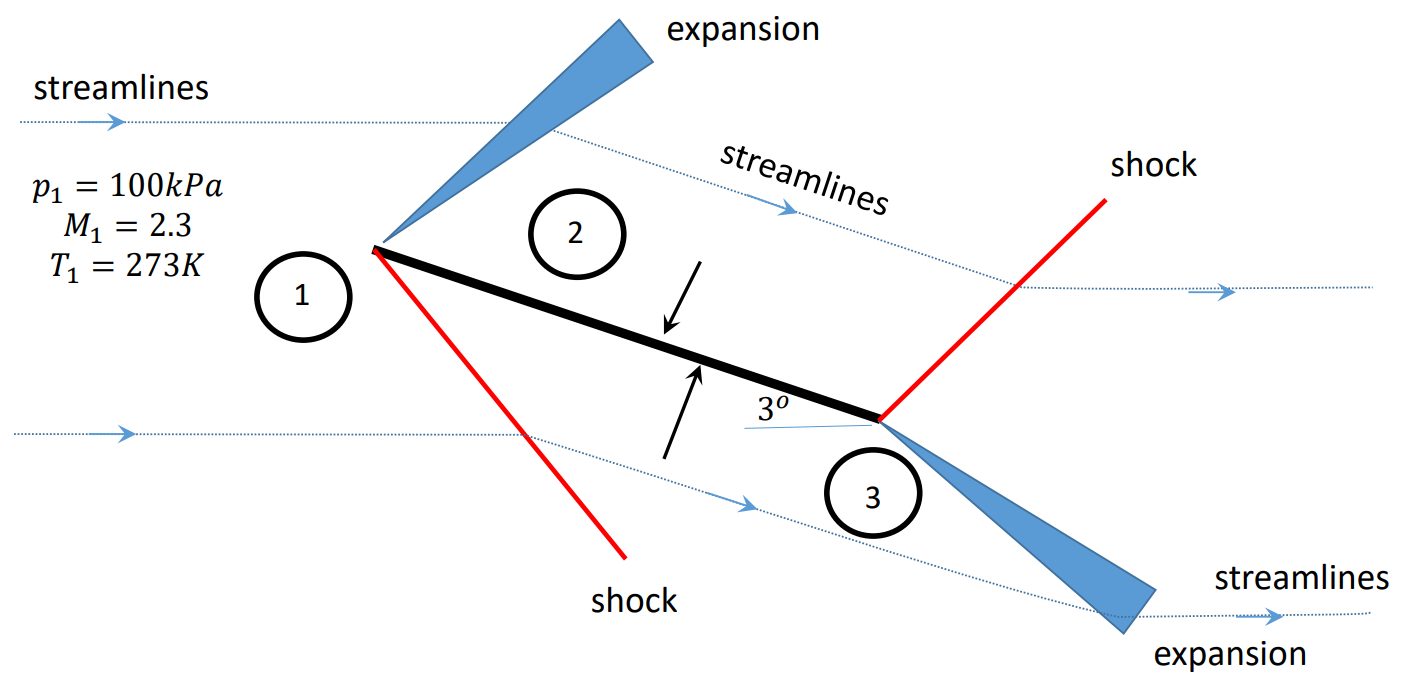
\includegraphics[width = 0.9\textwidth]{./img/diagram32.png}
\end{figure}
\subsection{Flat plate and Ellipse}
Lets consider a cylinder:
\begin{figure}[H]
  \centering
  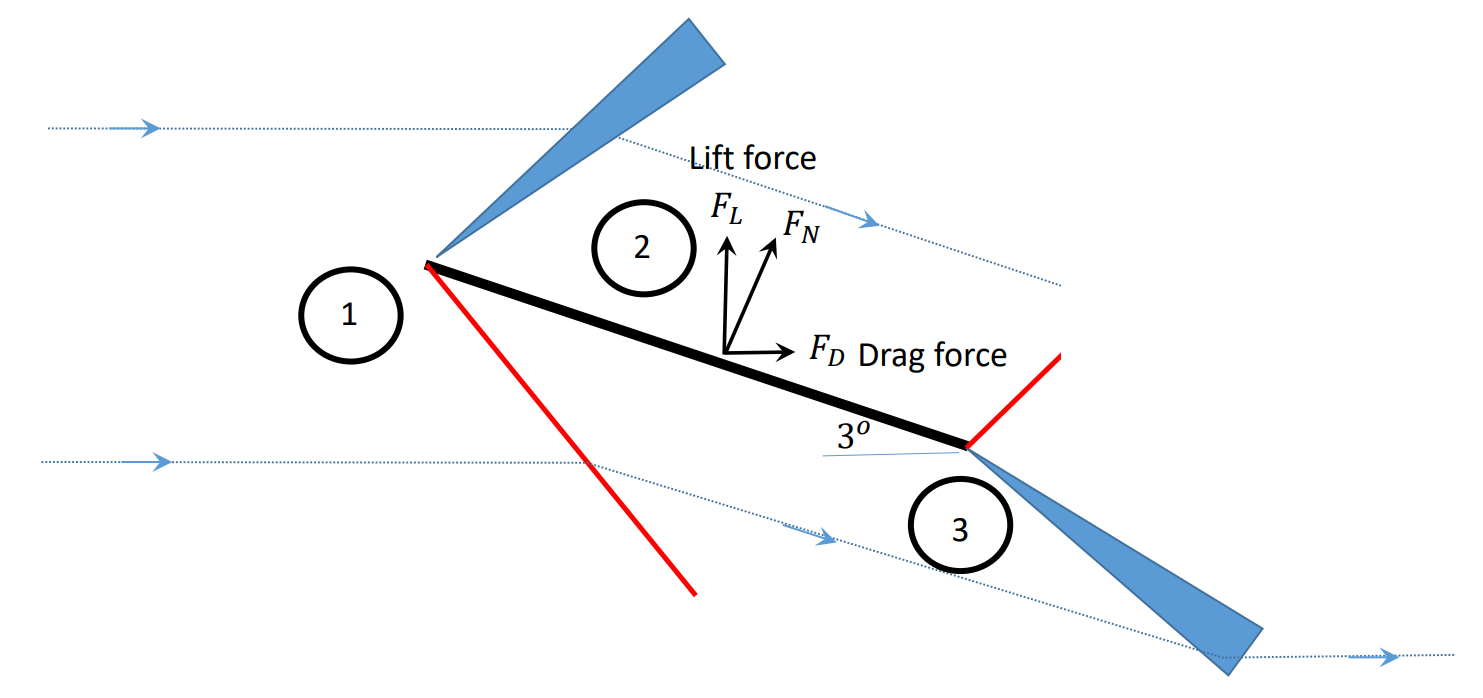
\includegraphics[width = 0.9\textwidth]{./img/diagram33.png}
\end{figure}
\begin{align}
  z & = R\cos{\theta} + Ri\sin{\theta}                                                                                                                       \\
  w & = G(z) = z + \frac{\lambda^2}{z}                                                                                                                       \\
    & =  R\cos{\theta} + Ri\sin{\theta} + \frac{\lambda^2}{R\cos{\theta} + Ri\sin{\theta}}                                                                   \\
    & = R\cos{\theta} + Ri\sin{\theta} + \frac{\lambda^2 (R\cos{\theta} - Ri\sin{\theta})}{(R\cos{\theta} + Ri\sin{\theta})(R\cos{\theta} - Ri\sin{\theta})} \\
    & = R\cos{\theta} + Ri\sin{\theta} + \frac{\lambda^2 (R\cos{\theta} - Ri\sin{\theta})}{R^2}                                                              \\
  w & = R\cos{\theta} \left(1 + \frac{\lambda^2}{R}\right) + Ri\sin{\theta} \left(1 - \frac{\lambda^2}{R}\right)
\end{align}
When $\lambda = R$, we achieve a flat plate transformation as our imaginary term is always 0. When $\lambda \neq R$, we achieve an elliptical shape.
\begin{figure}[H]
  \centering
  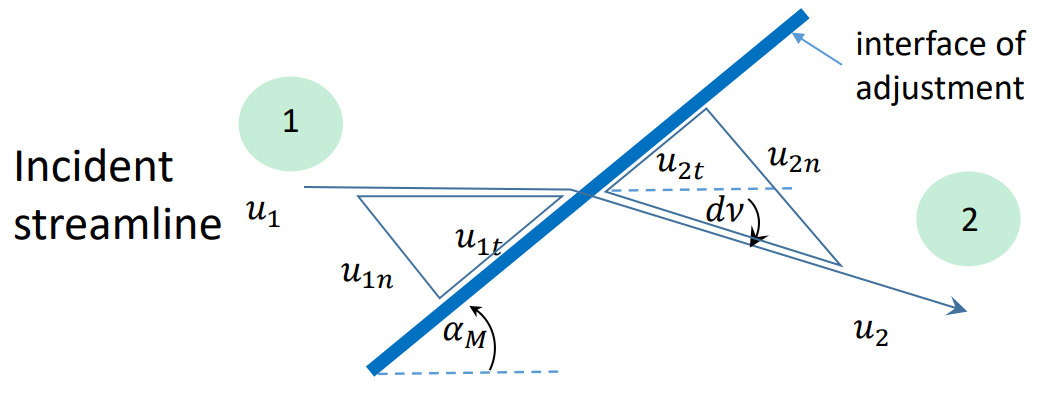
\includegraphics[width = 0.9\textwidth]{./img/diagram34.png}
\end{figure}
\subsection{Aerofoils}
We can further refine our conformal mapping by adding two elements to our equation, $x_c$ and $y_c$. These two terms effect the center of the cylinder in $x$ and $y$.
\begin{gather}
  w = G(z) = z + \frac{\lambda^2}{z}\\
  \lambda = R - \sqrt{x_c^2 + y_c^2}\\
  z = x + x_c + (y + y_c)i \rightarrow w = \zeta + \xi i
\end{gather}
Mapping these into their respective planes:
\begin{align}
  x_c & \neq 0 \\
  y_c & = 0
\end{align}
\begin{figure}[H]
  \centering
  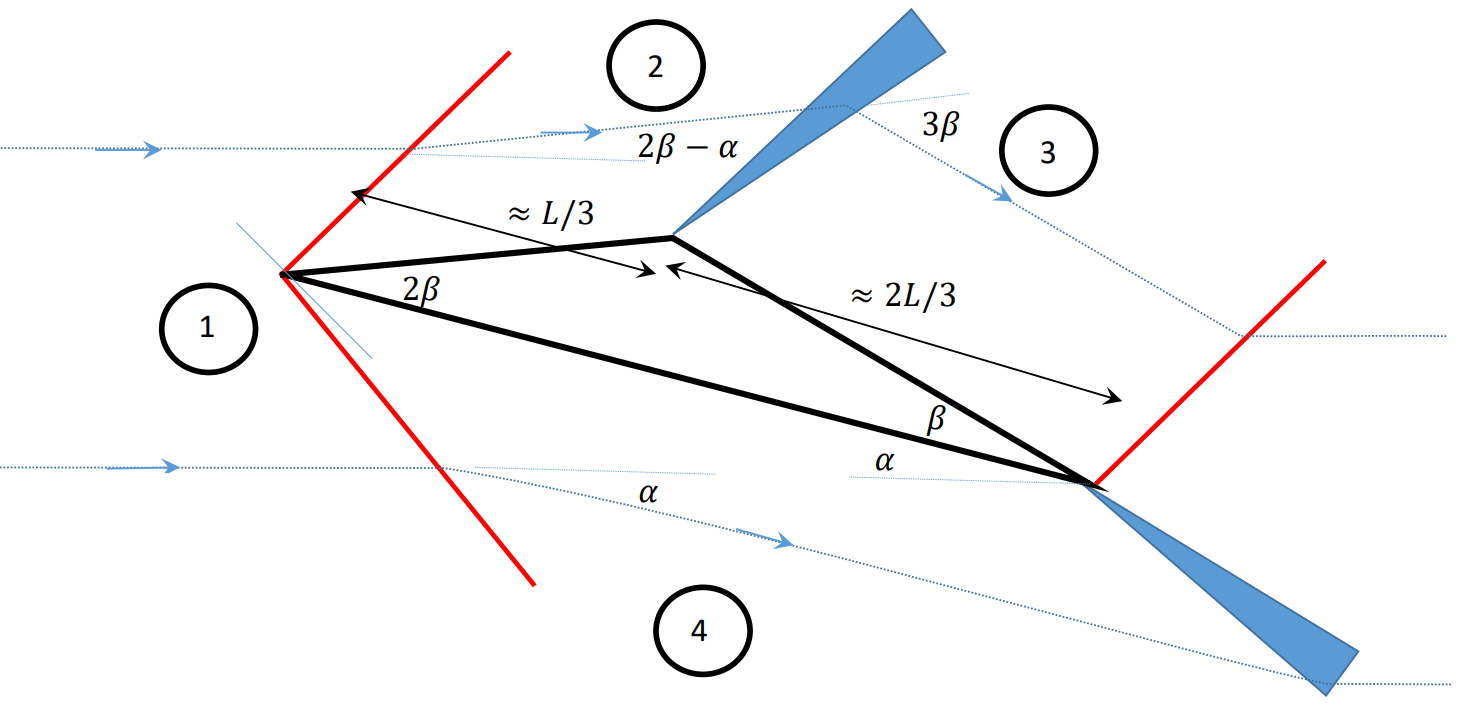
\includegraphics[width = 0.7\textwidth]{./img/diagram35.png}
\end{figure}
\begin{align}
  x_c & \neq 0 \\
  y_c & \neq 0
\end{align}
\begin{figure}[H]
  \centering
  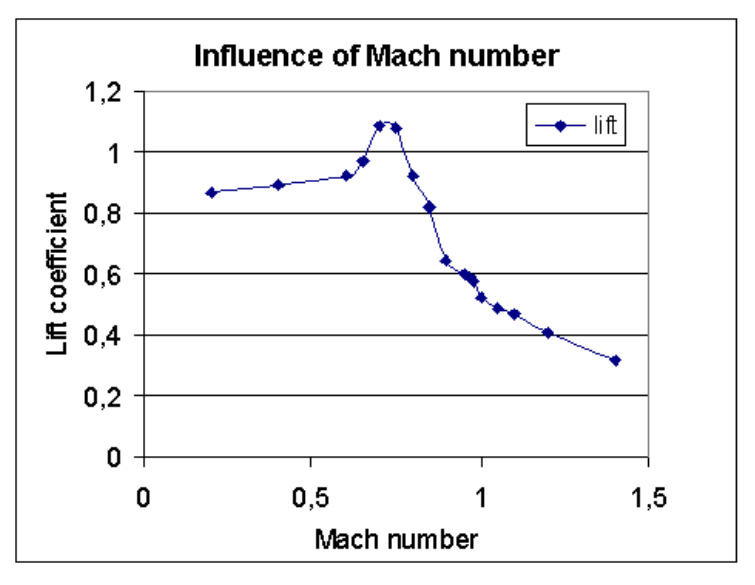
\includegraphics[width = 0.7\textwidth]{./img/diagram36.png}
\end{figure}
\subsection{Cambered airfoil}
\begin{figure}[H]
  \centering
  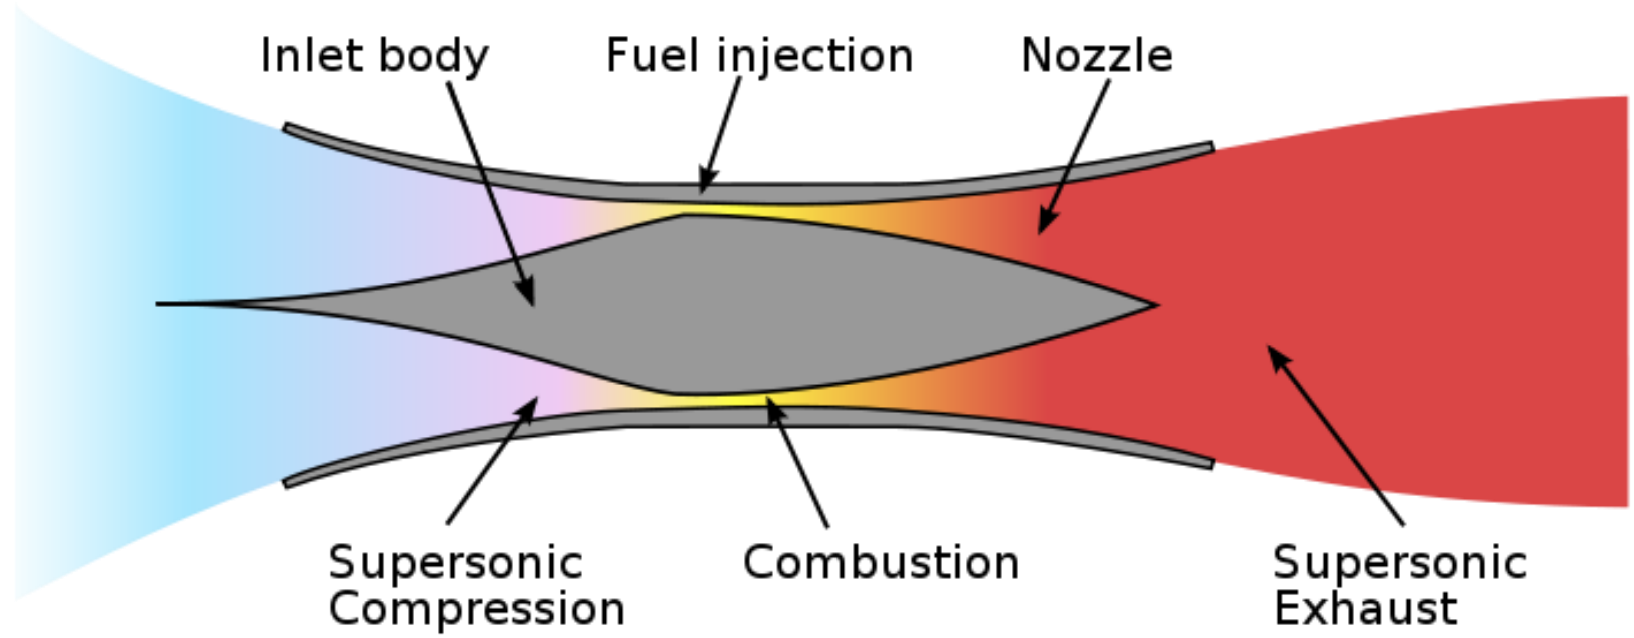
\includegraphics[width = \textwidth]{./img/diagram44.png}
  \caption{$x_c = -0.1$, $y_c = 0.1$, $sin{\beta} = \frac{y_c}{R}$}
\end{figure}
\section{Uniform stream + circulation}
What is the correct relationship between the circulation and the angle of incidence?
\begin{align}
  \Gamma                           & = f(\alpha)                                                                                                               \\
  \textrm{Stagnation points: } u_r & = 0, \ u_\theta = 0                                                                                                       \\
  \phi                             & = V_\infty r \cos{(\theta - \alpha)}\left(1 + \frac{R^2}{r^2}\right) - \frac{\Gamma}{2\pi}\theta                          \\
  \psi                             & = V_\infty r \sin{(\theta - \alpha)}\left(1 - \frac{R^2}{r^2}\right) + \frac{\Gamma}{2\pi} \log{\left(\frac{r}{R}\right)}
\end{align}
\begin{figure}[H]
  \centering
  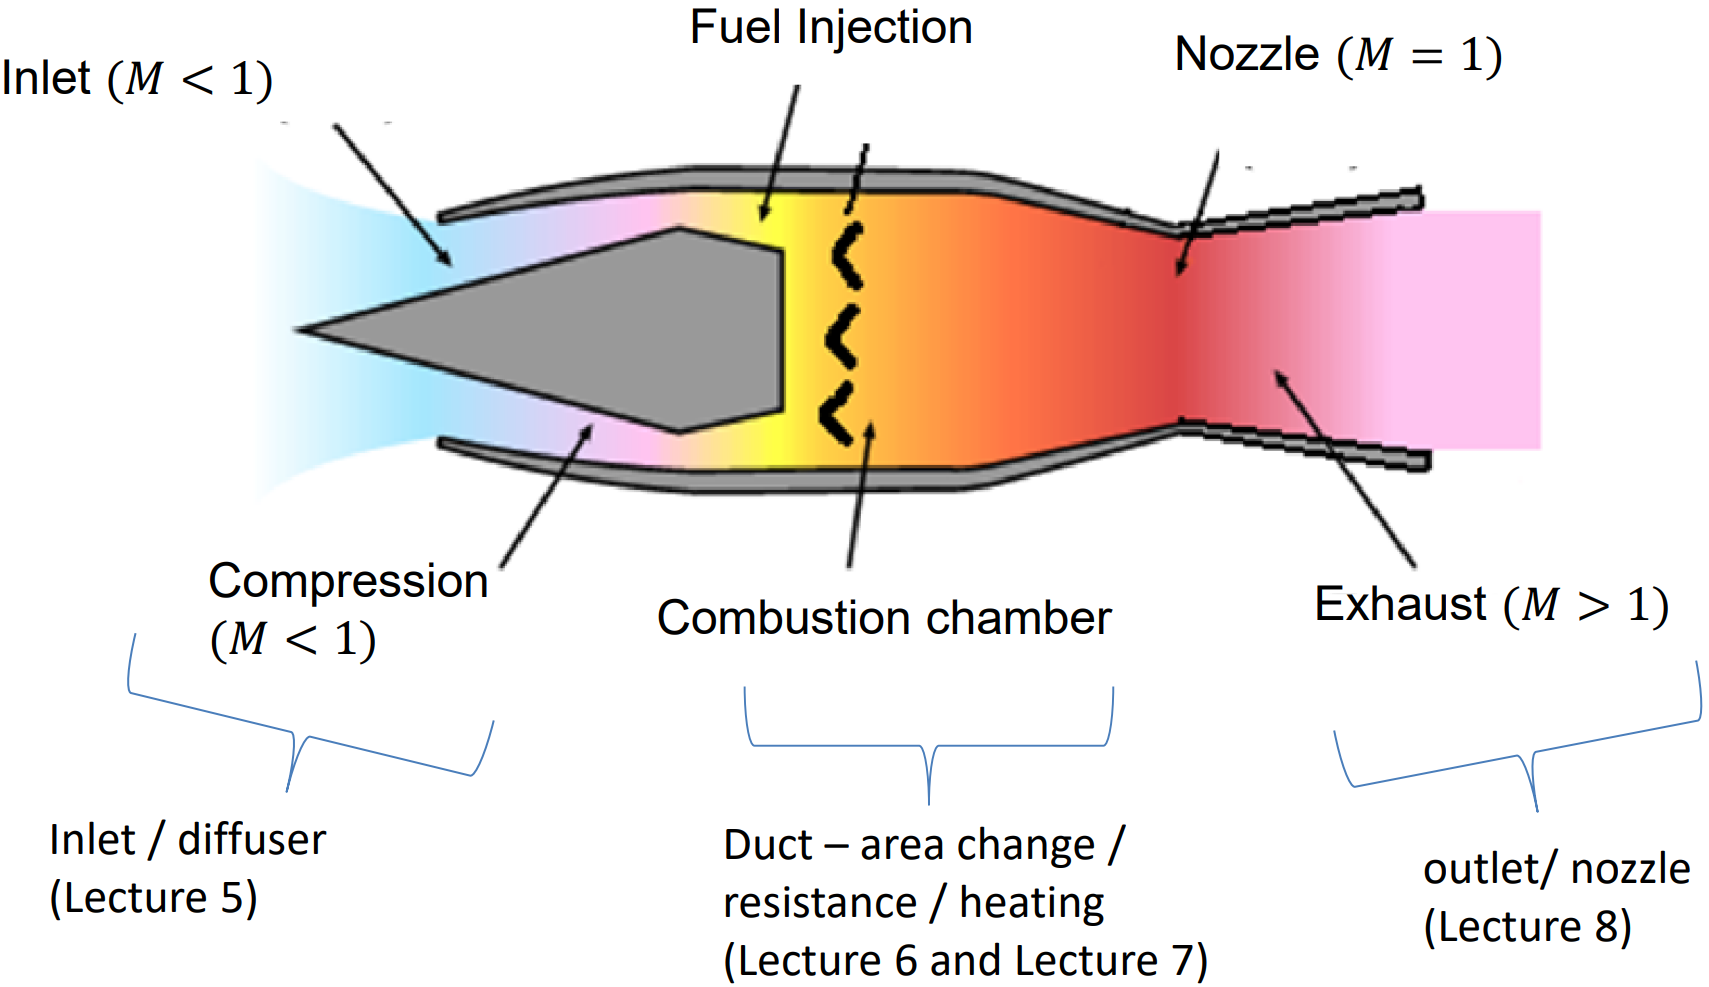
\includegraphics[width = 0.7\textwidth]{./img/diagram37.png}
\end{figure}
\section{Kutta condition}
I can apply the Joukowsky Transformation to the streamlines around the cylinder and obtain the streamlines around the airfoil. However I need to carefully select the circulation, $\Gamma$.
\begin{figure}[H]
  \centering
  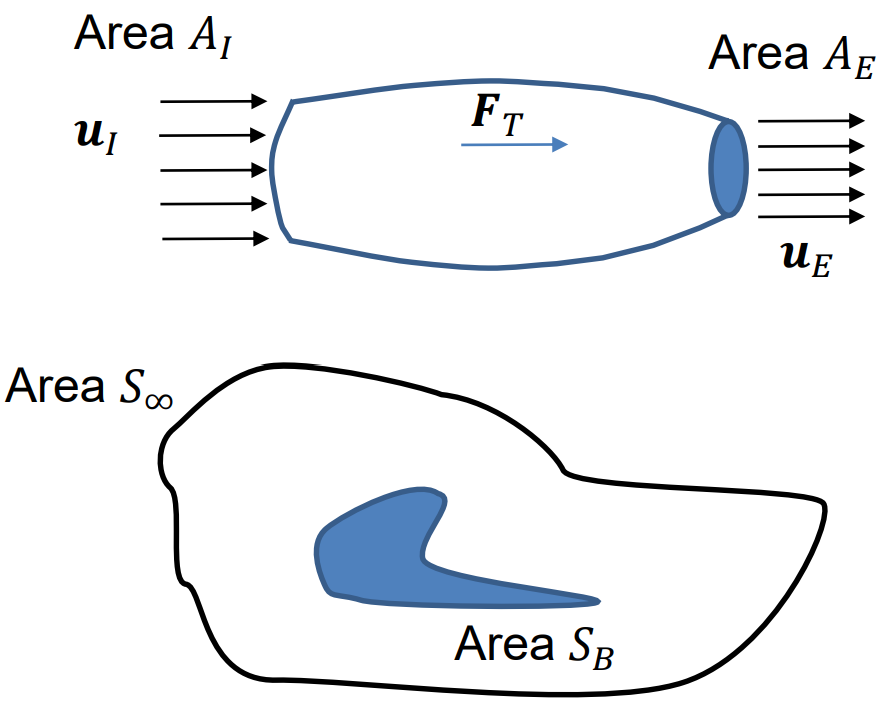
\includegraphics[width = 0.9\textwidth]{./img/diagram38.png}
\end{figure}
We can see that this streamline is unrealistic. This is because to curl around the trailing edge cusp, the speed goes to infinity. This is clearly impossible and flow separation would occur instead. This is the wrong circulation value for the given angle of incidence.
\begin{figure}[H]
  \centering
  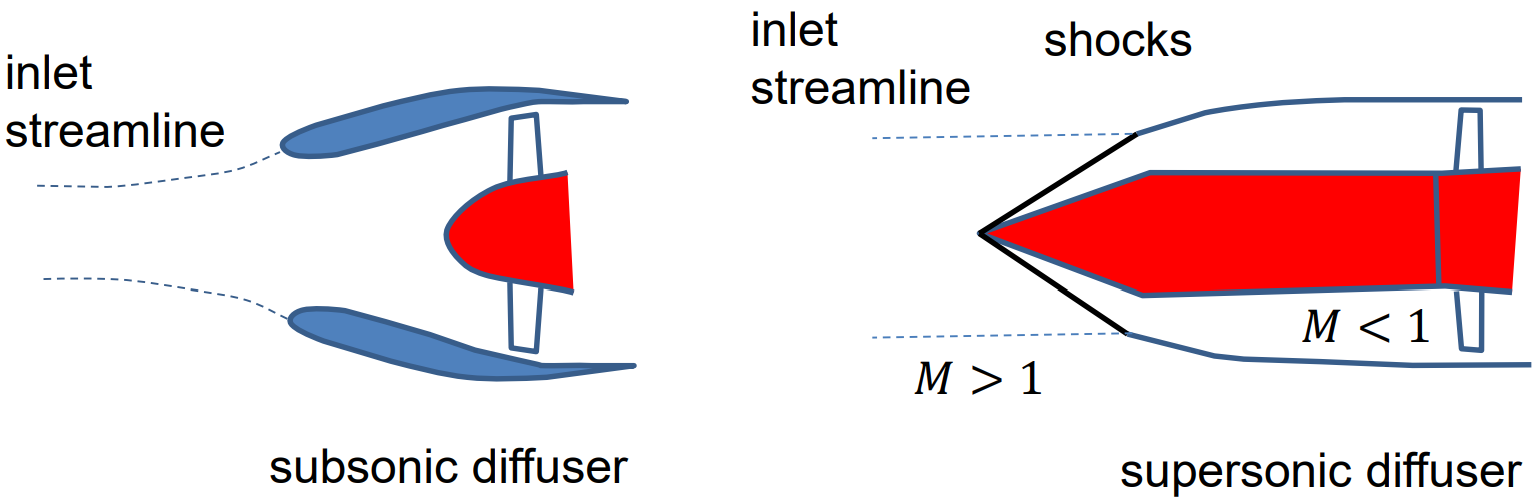
\includegraphics[width = 0.9\textwidth]{./img/diagram39.png}
\end{figure}
This streamline is more realistic as the velocity is parallel to the trailing edge cusp and its component in the vertical direction is zero. This circulation can be used to predict the lift $F_L$ but still predicts no drag $(F_D = 0)$. The next question is how do we achieve this mapping?
\begin{figure}[H]
  \centering
  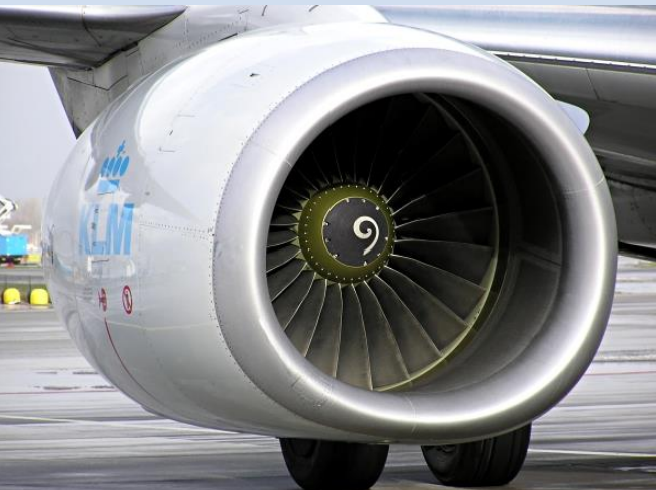
\includegraphics[width = 0.9\textwidth]{./img/diagram40.png}
\end{figure}
We can see here that for a given angle of coincidence, the circulation has to be selected by imposing that the back stagnation point (red circle) and the point corresponding to the airfoil trailing edge (black circle) coincide.
\begin{align}
  \phi & = V_\infty r \cos{(\theta - \alpha )}\left(1 + \frac{R^2}{r^2}\right) - \frac{\Gamma}{2\pi}\theta                         \\
  \psi & = V_\infty r \sin{(\theta - \alpha)}\left(1 - \frac{R^2}{r^2}\right) + \frac{\Gamma}{2\pi} \log{\left(\frac{r}{R}\right)}
\end{align}
Velocity components:
\begin{align}
  u_r      & = \frac{1}{r} \frac{\partial \psi}{\partial \theta} = V_\infty r \cos{(\theta - \alpha)}\left(1-\frac{R^2}{r^2}\right)            \\
  u_\theta & = - \frac{\partial \psi}{\partial r} = -V_\infty \sin{(\theta - \alpha)} \left(1 + \frac{R^2}{r^2}\right) - \frac{\Gamma}{2\pi r}
\end{align}
On the cylinder $r = R$:
\begin{align}
  u_r      & = 0                                                        \\
  u_\theta & = -2V_\infty \sin{(\theta-\alpha)} - \frac{\Gamma}{2\pi R}
\end{align}
Kutta condition:
\begin{align}
  u_\theta (\theta = 0)                     & = 0                           \\
  \Gamma = -4\pi V_\infty R \sin{(-\alpha)} & = 4\pi V_\infty R\sin{\alpha}
\end{align}
For a cambered aerofoil:
\begin{align}
  u_\theta (\theta = -\beta) & = 0                                                                                \\
  \Gamma                     & = -4\pi V_\infty R \sin{(-\beta -\alpha)} = 4\pi V_\infty R \sin{(\beta + \alpha)}
\end{align}
\section{Aerofoil lift}
\begin{figure}[H]
  \centering
  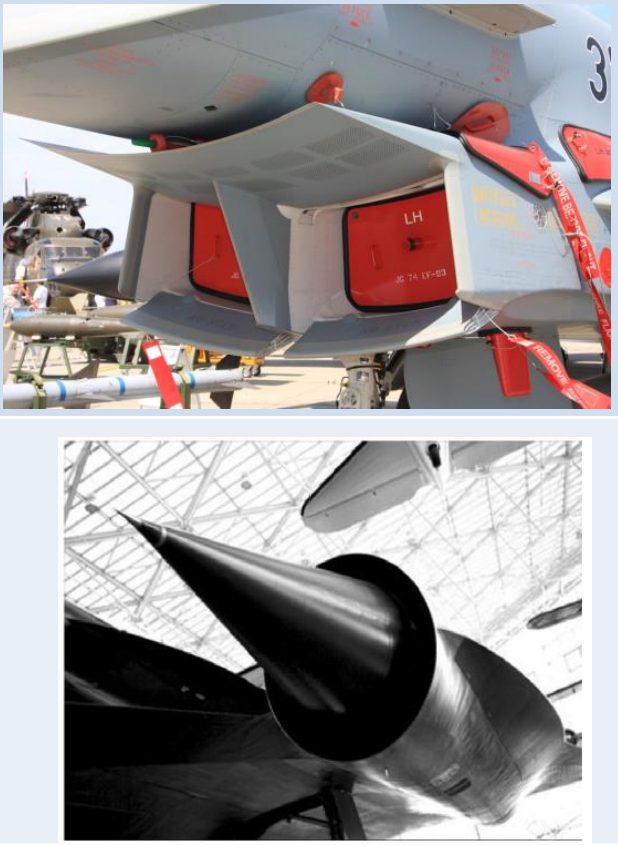
\includegraphics[width = 0.6\textwidth]{./img/diagram41.png}
\end{figure}
The lift is given by:
\begin{align}
  L = \rho V \Gamma = 4 \rho \pi V_\infty^2 R \sin{\alpha}
\end{align}
The lift coefficient is:
\begin{align}
  c_L = \frac{L}{\frac{1}{2}\rho V_\infty^2 c} = 9\pi \frac{R}{c}\sin{\alpha}
\end{align}
Flow is inviscid so zero drag.
\section{Flow past an Aerofoil}
\subsection{How was the circulation created?}
When an airfoil is still on the ground there is no flow and total circulation is zero. As soon as the airfoil takes off a negative circulation is created at the back oft he airfoil and a positive one is stored within the airfoil boundary layer.
\subsection{Stalling}
If the angle of attack becomes too great and boundary layer separation occurs on the top of the aerofoil the pressure pattern will change dramatically. In such a case, the lift component is insufficient to overcome the weight of the aircraft and disaster is imminent. This phenomenon is known as stalling. When stalling occurs, all, or most, of the 'suction' pressure is lost and the plane will suddenly drop from the sky. The solution to this is to put the plane into a dive to regain the boundary layer. A transverse lift force is then exerted on the wing which gives the pilot some control and allows the plane to be pulled out of the dive.
\begin{figure}[H]
  \centering
  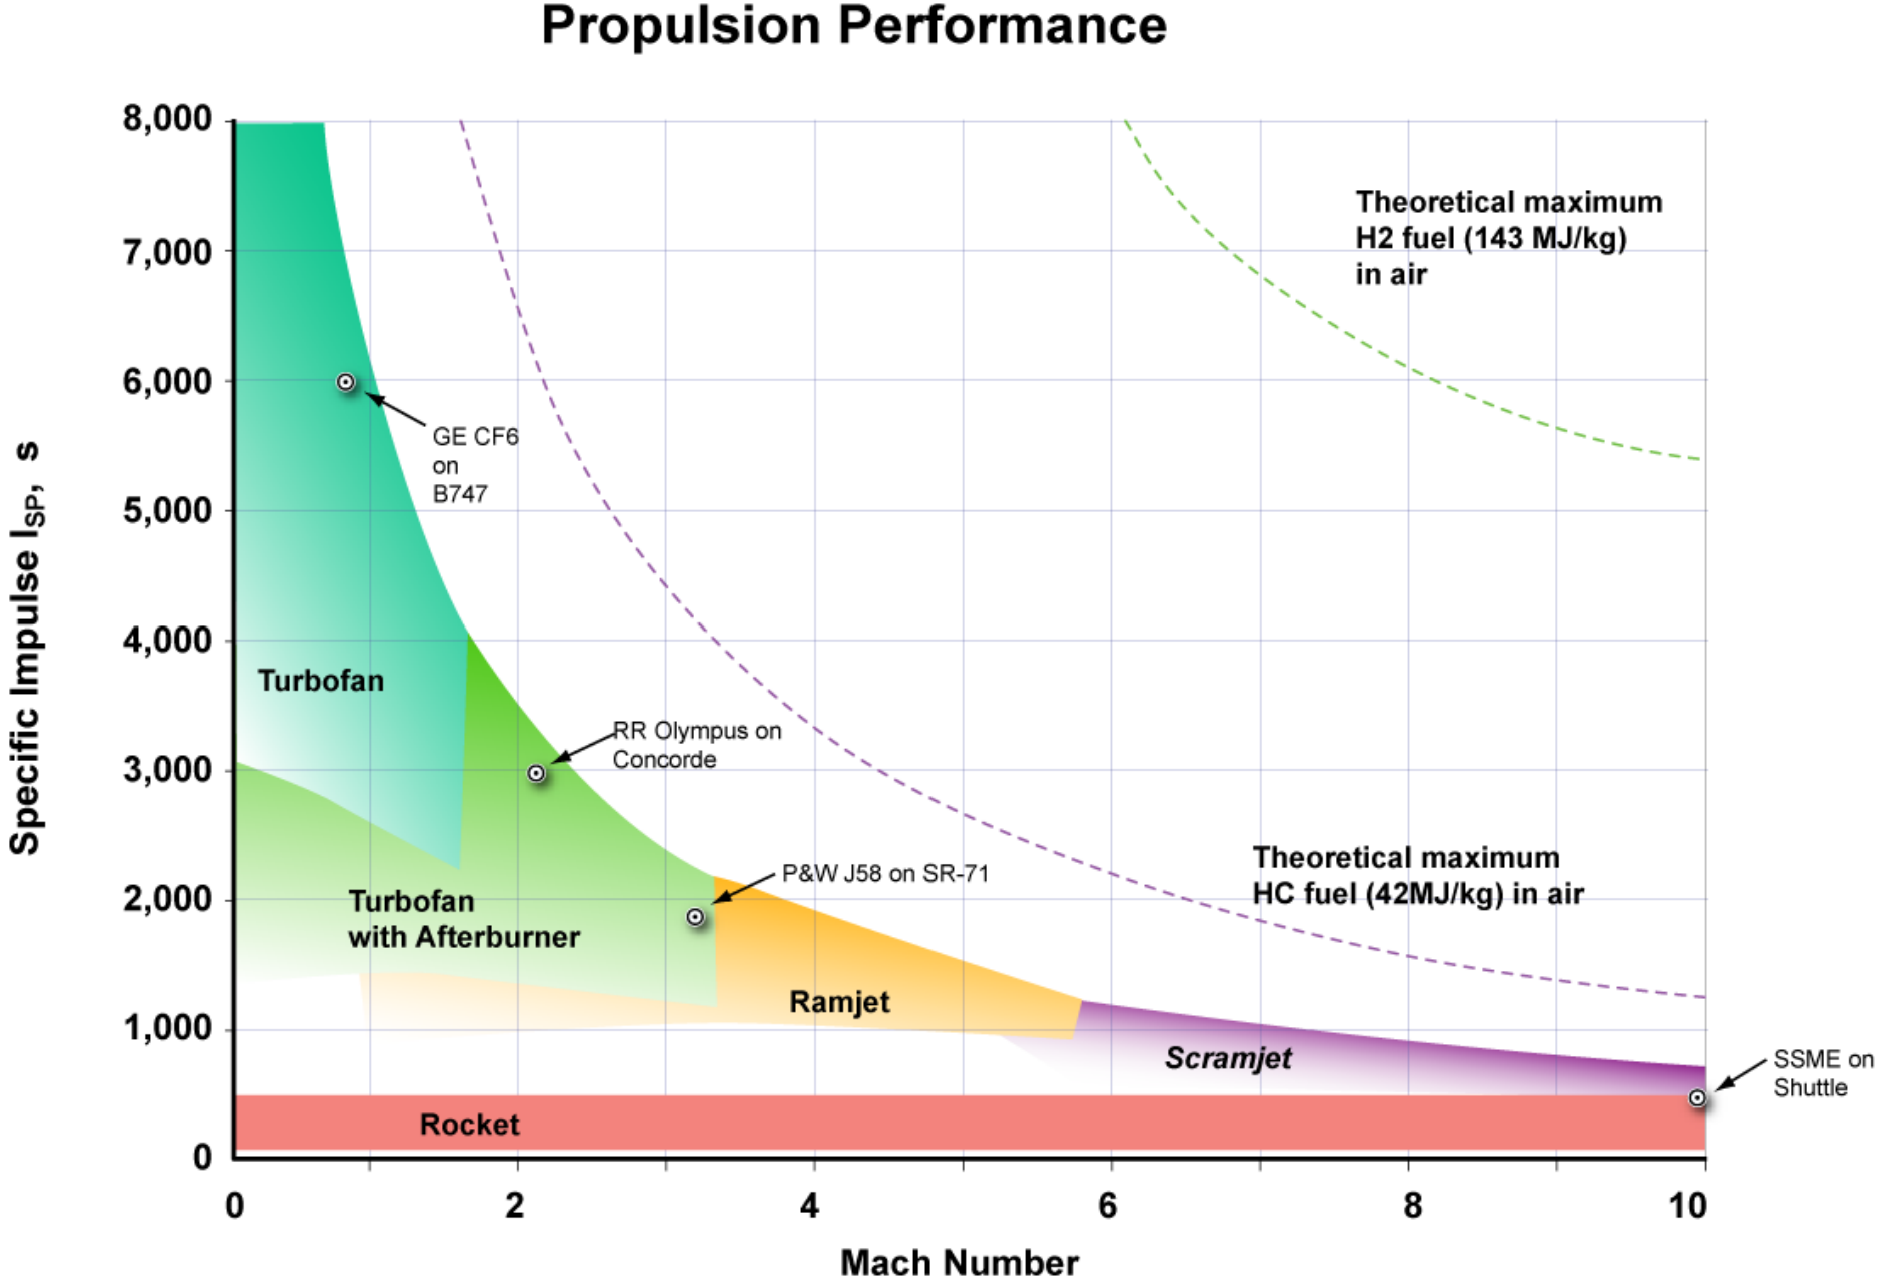
\includegraphics[width = 0.9\textwidth]{./img/diagram42.png}
\end{figure}
Boundary layer separation occurs on the upper surface (where the adverse pressure gradients are large) amd produces a different $c_p$ distribution from the unseparated case. As skin friction is predominant for the unstalled wing, the profile drag is sensitive to any increase in form drag.
\begin{itemize}
  \item At a small angle of attack $a$: separation is close to trailing edge, wake is thin, low form of drag
  \item As the angle of attack $a$ increases: separation moves along the top of the aerofoil, wake width increases, form drag increases
  \item The critical angle of attack $a_{crit}$: value of $a$ form maximum $c_L$, stall angle
  \item If the angle of attack $a > a_{crit}$: separation from most of the upper surface, wider wake with turbulence, considerable form drag
\end{itemize}
The exact value of the critical angle of attack depends on the type and shape of the aerofoil.
\begin{figure}[H]
  \centering
  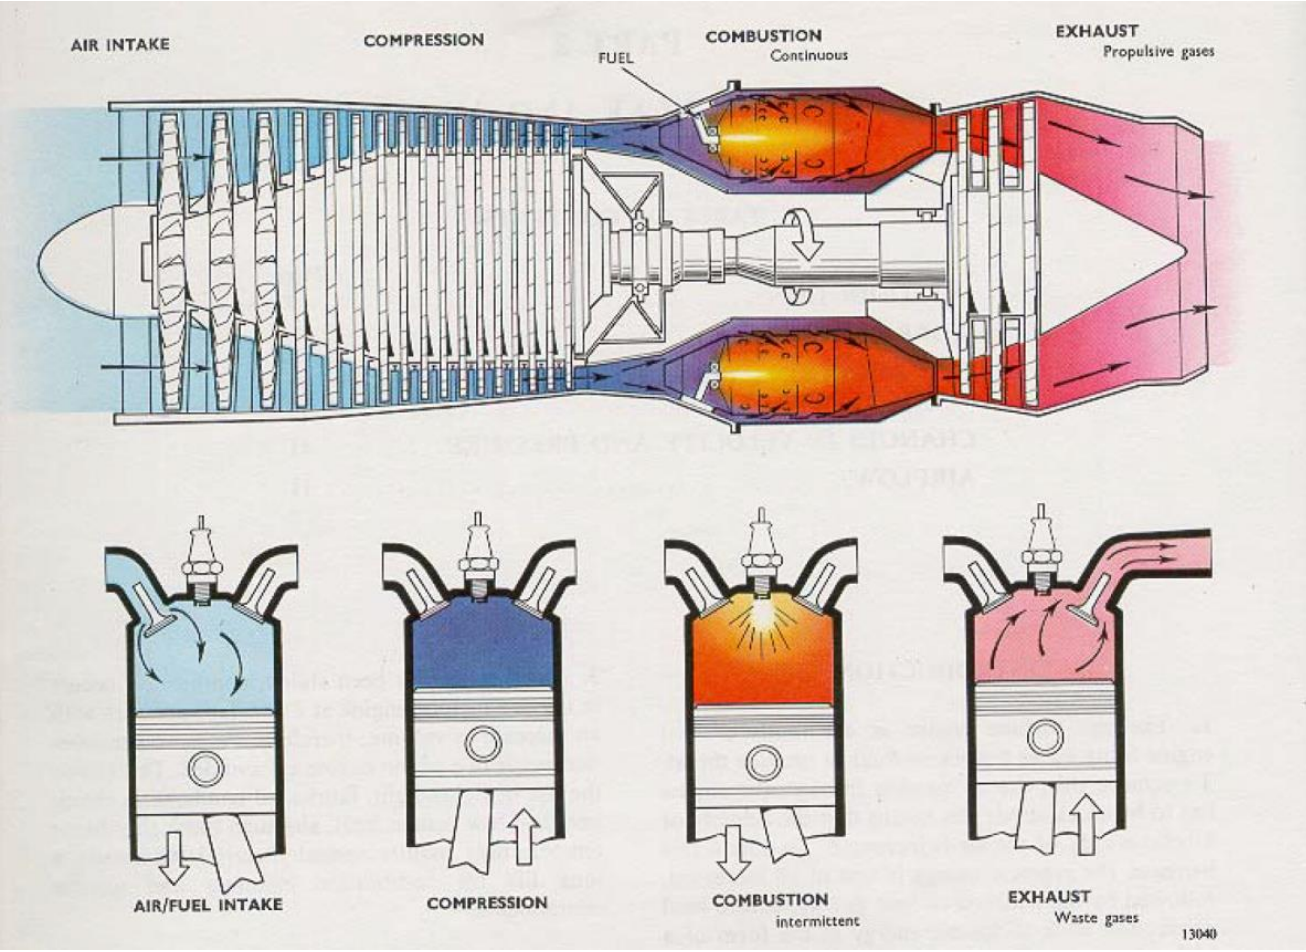
\includegraphics[width = 0.9\textwidth]{./img/diagram43.png}
\end{figure}
\section{Form drag and skin friction}
\begin{figure}[H]
  \centering
  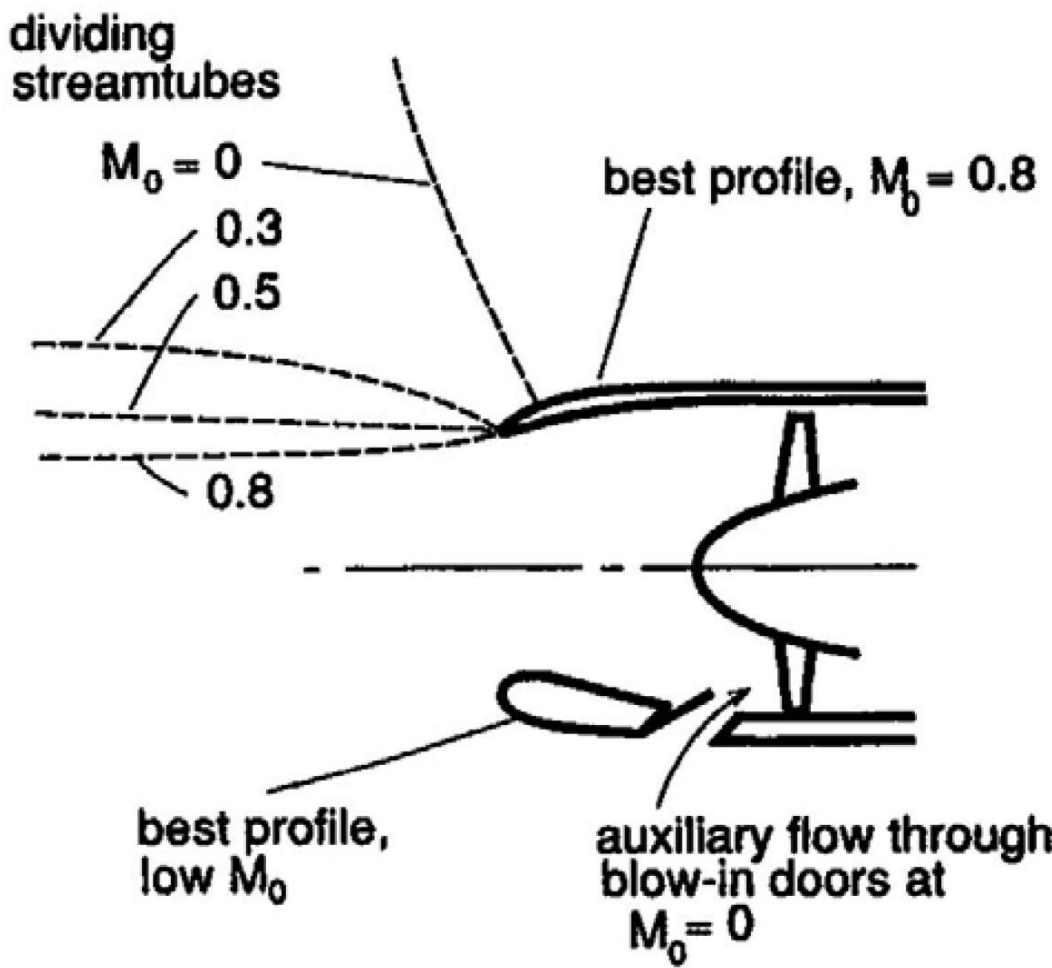
\includegraphics[width = 0.6\textwidth]{./img/diagram45.png}
\end{figure}
Force due to pressure $p$ on element of surface area $\dif s$ is $p \dif s$. The force $p \dif s$ has a component in the stream direction and if this component is integrated over the whole body surface, it gives the drag due to pressure distribution or the form drag. Form drag is the resultant of the forces normal to the surface (pressure distribution: normal stresses). The same element of area $\dif s$ experiences a shear stress $\tau_w$ due ot the velocity of the gradient normal to the surface and the associated shear force is $\tau_w \dif s$. This also has a component in the stream direction which when integrated over the body surface gives the drag due due to skin friction. Skin friction drag is resultant of forces tangential to the surface (shear stresses).
\section{Total drag}
Total drag (also known as profile drag) is given by:
\begin{equation}
  \textrm{Total drag} = \textrm{Form drag} + \textrm{Skin friction}
\end{equation}
Separation is what leads to large form drag. The benefits of streamlining can be considerable.
\begin{figure}[H]
  \centering
  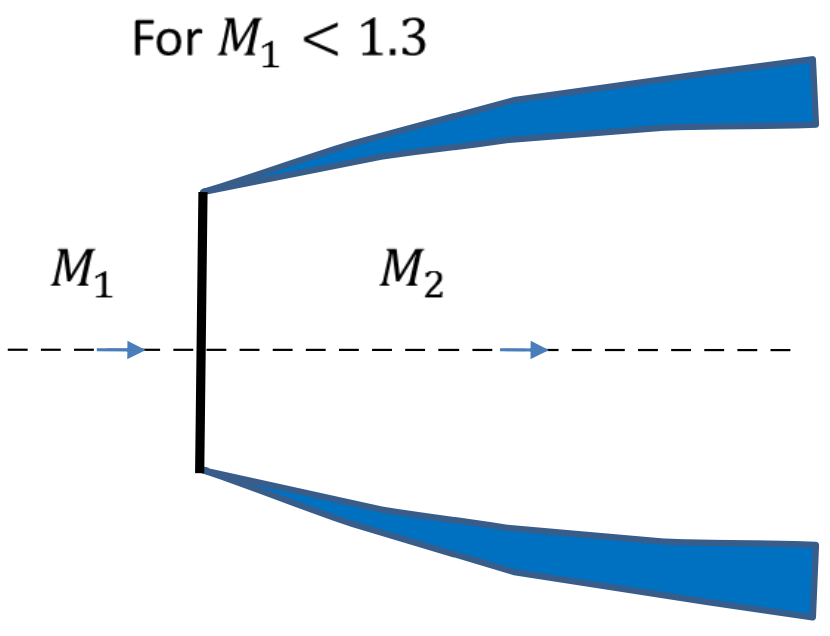
\includegraphics[width = 0.6\textwidth]{./img/diagram46.png}
\end{figure}
\begin{figure}[H]
  \centering
  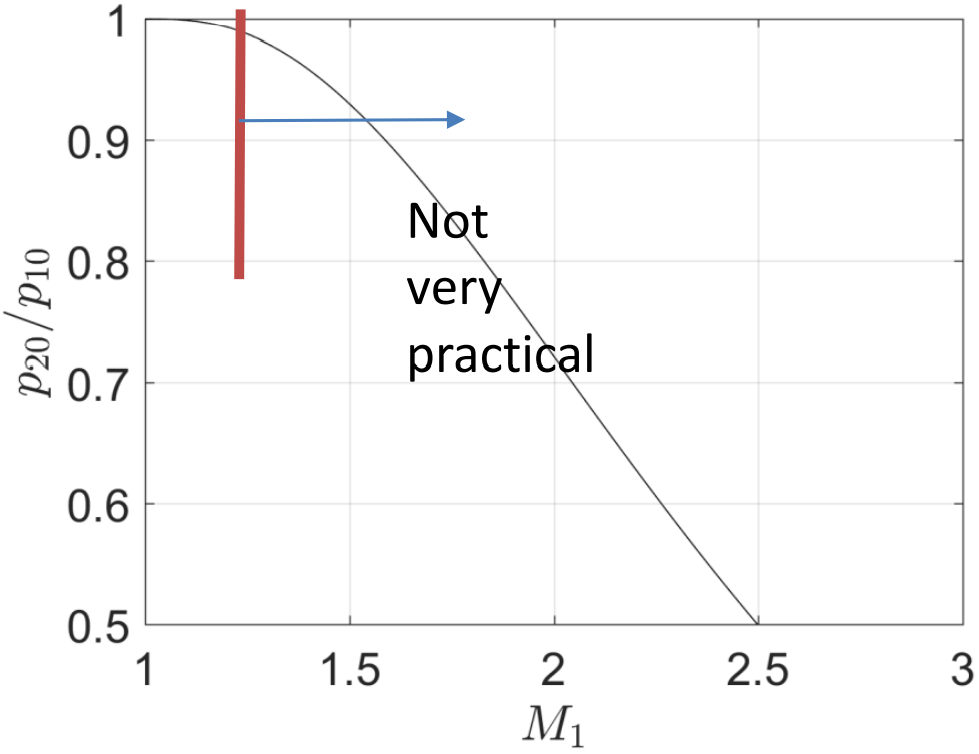
\includegraphics[width = \textwidth]{./img/diagram47.png}
\end{figure}